%%%%%%%%%%%%%%%%%%%%%%%%%%%%%%%%%%%%%%%%%
% Beamer Presentation
% LaTeX Template
% Version 1.0 (10/11/12)
%
% This template has been downloaded from:
% http://www.LaTeXTemplates.com
%
% License:
% CC BY-NC-SA 3.0 (http://creativecommons.org/licenses/by-nc-sa/3.0/)
%
%%%%%%%%%%%%%%%%%%%%%%%%%%%%%%%%%%%%%%%%%

%----------------------------------------------------------------------------------------
%   PACKAGES AND THEMES
%----------------------------------------------------------------------------------------

\documentclass{beamer}

\mode<presentation> {

% The Beamer class comes with a number of default slide themes
% which change the colors and layouts of slides. Below this is a list
% of all the themes, uncomment each in turn to see what they look like.

\usetheme{Madrid}

% As well as themes, the Beamer class has a number of color themes
% for any slide theme. Uncomment each of these in turn to see how it
% changes the colors of your current slide theme.

\usecolortheme{seagull}

%\setbeamertemplate{footline} % To remove the footer line in all slides uncomment this line
%\setbeamertemplate{footline}[page number] % To replace the footer line in all slides with a simple slide count uncomment this line

%\setbeamertemplate{navigation symbols}{} % To remove the navigation symbols from the bottom of all slides uncomment this line
}

\usepackage{graphicx} % Allows including images
\usepackage{booktabs} % Allows the use of \toprule, \midrule and \bottomrule in tables


\usepackage[ final ]{pdfpages}
%----------------------------------------------------------------------------------------
%   TITLE PAGE
%----------------------------------------------------------------------------------------

\title[Software ontwerp: iteratie 1]{Software ontwerp: iteratie 1 (groep 8)} % The short title appears at the bottom of every slide, the full title is only on the title page

\author[Groep 8]{\\
        Andr\'e Jacobs \\
        Menno Keustermans\\
        Bruno Lannoo \\
        Thomas Marcelis} % Your name
\institute[KULeuven] % Your institution as it will appear on the bottom of every slide, may be shorthand to save space
{\\ % Your institution for the title page
\medskip
\textit{} % Your email address
}
\date{} % Date, can be changed to a custom date
\usepackage{graphicx}
\usepackage{caption}
\usepackage{subcaption}
\begin{document}

\begin{frame}
\titlepage % Print the title page as the first slide
\end{frame}


%----------------------------------------------------------------------------------------
%   PRESENTATION SLIDES
%----------------------------------------------------------------------------------------

%----------------------------------------------------------------------------------------
%   Packages overzicht:
%       In src zijn er 4 packages:
%       
%       Front-end : user interface
%                   -> gebruikt exception, parser en taskmanager
%       Back-end : taskManager
%----------------------------------------------------------------------------------------

\begin{frame}
\frametitle {Packages: overzicht}
\begin{figure}
\centering
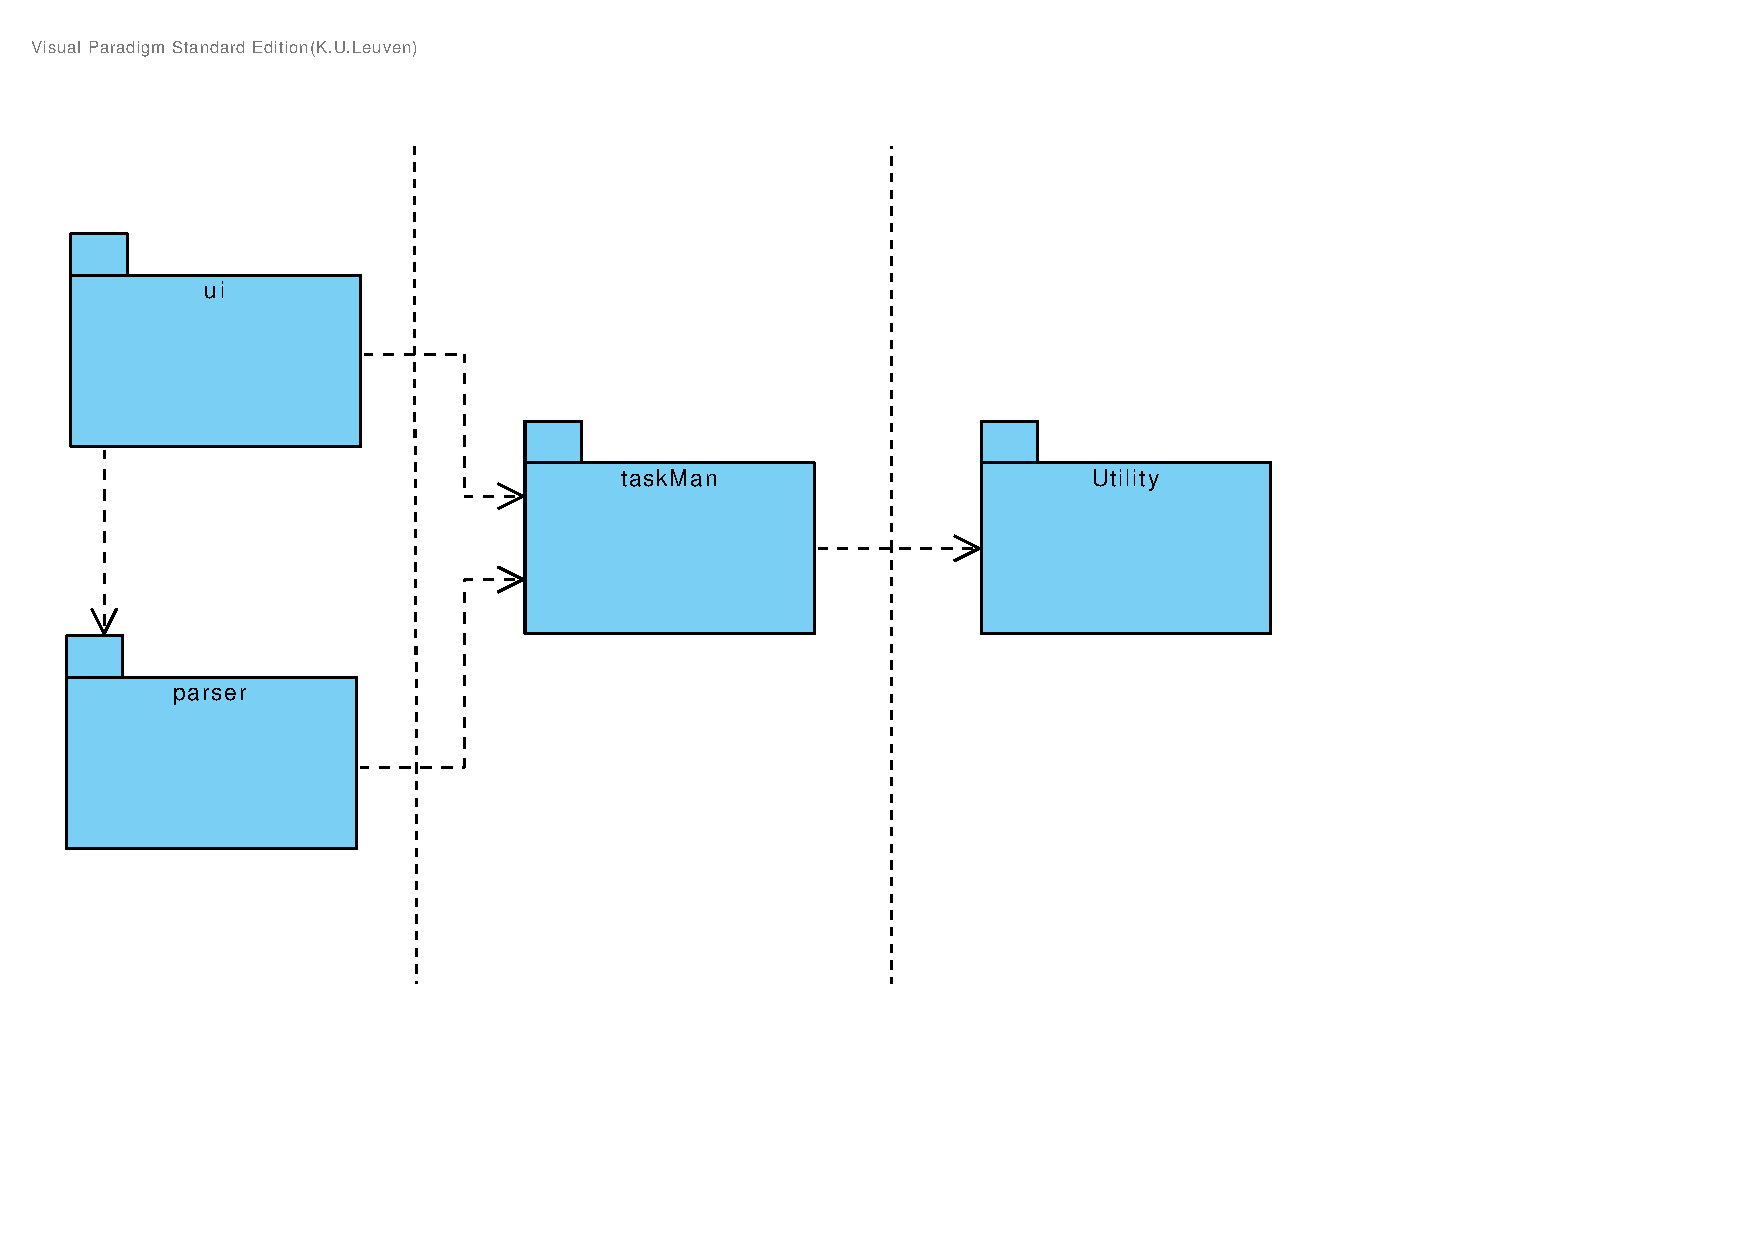
\includegraphics[width=1\textwidth]{figures/package_overview}
\caption{Test}
\end{figure}
\end{frame}

%----------------------------------------------------------------------------------------
%   Class diagram overzicht: (back-end)
%       Project-controller heeft overzicht over alle projecten en bevat
%       de interne klok van het systeem
%
%       Project heeft overzicht van alle taken
%
%       Taken
%
%----------------------------------------------------------------------------------------

\begin{frame}
\frametitle {Class diagram: overzicht}
\vspace{-1.4cm}
\begin{figure}
\centering
\begin{center}
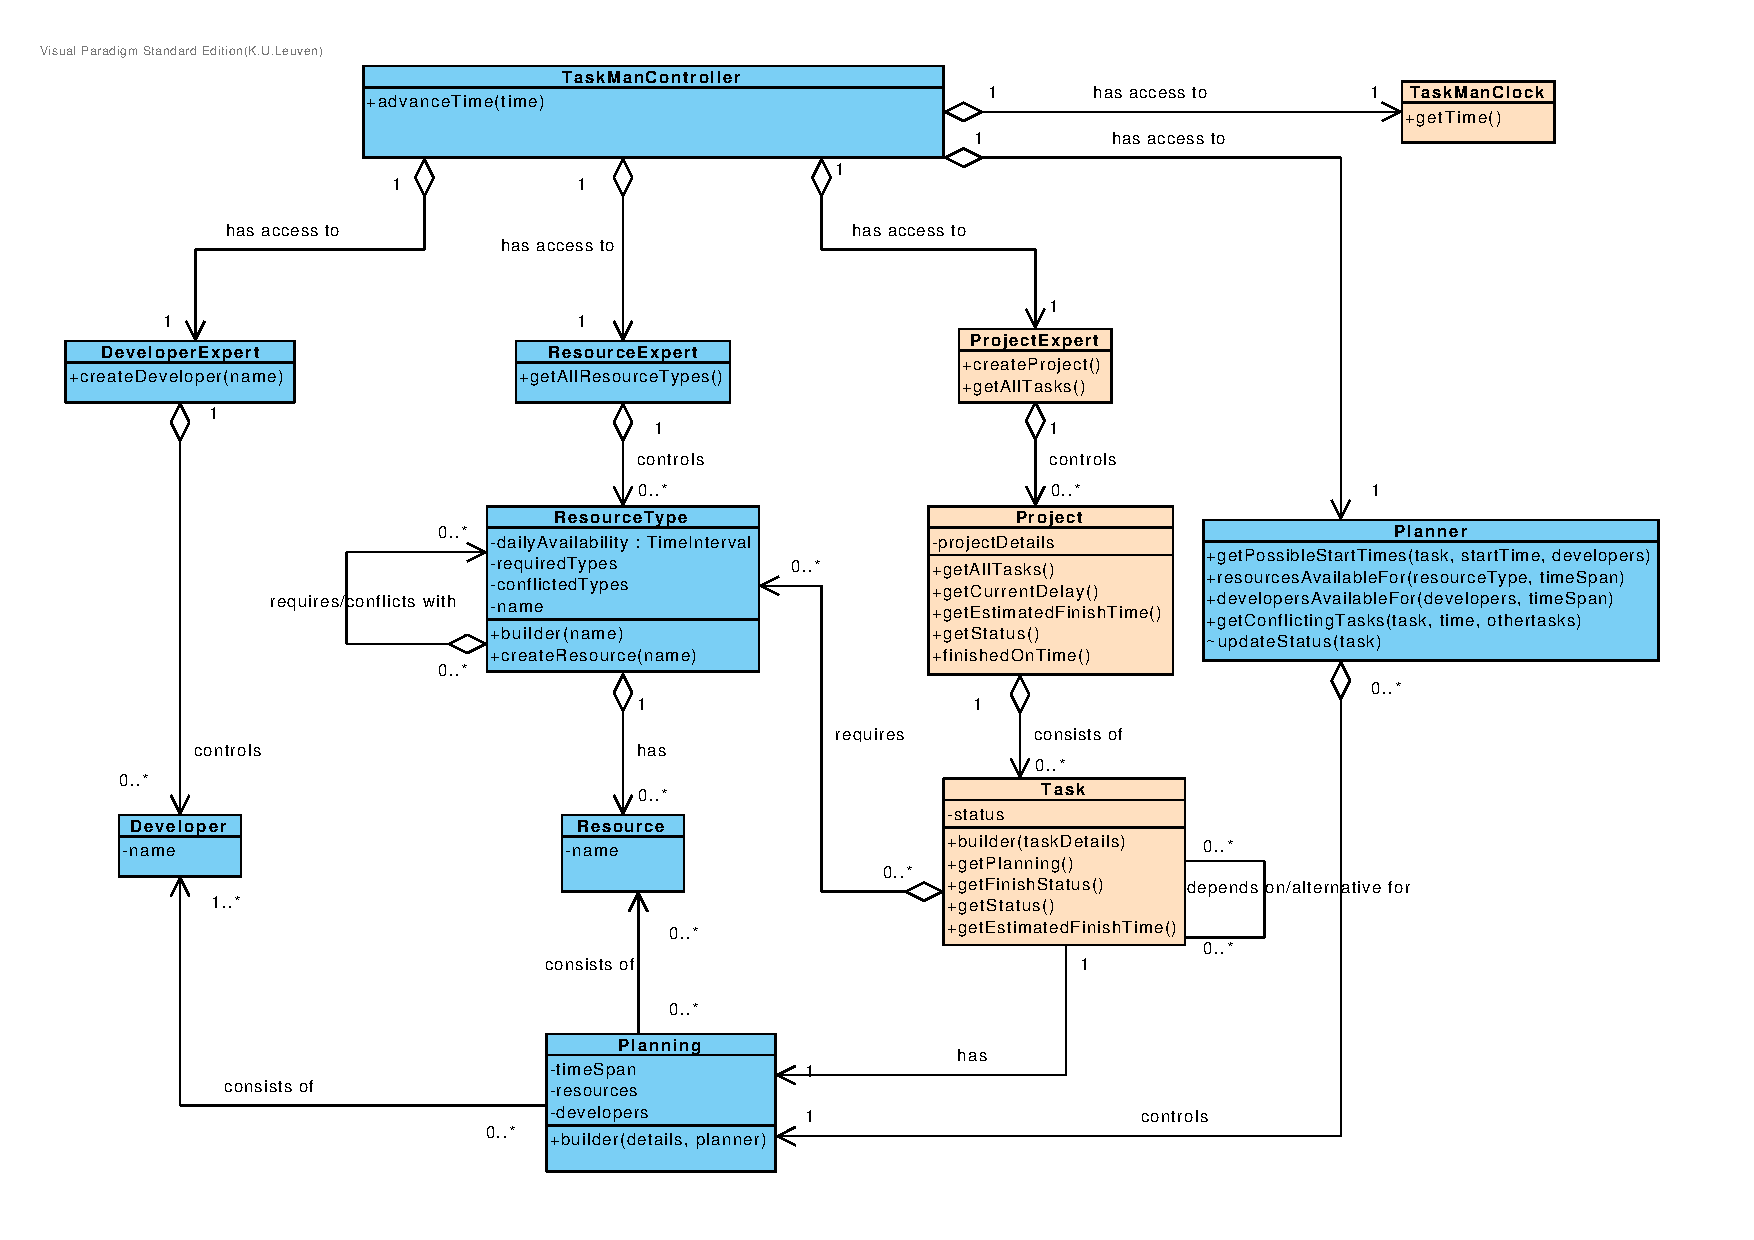
\includegraphics[width=1.05\textwidth]{figures/Class_diagram_iteratie2.pdf}
\end{center}

\end{figure}
\end{frame}

%----------------------------------------------------------------------------------------
%   ProjectController (discussion GRASP)
%       Information expert
%           Verantwoordelijkheden:
%               - houdt lijst van projecten bij
%               - houdt ook de klok bij
%
%           Creator:
%               Verantwoordelijkheden: 
%               - Maakt elk project aan.
%   
%           Controller:
%               Aanspreekpunt voor alle informatie
%
%----------------------------------------------------------------------------------------

\begin{frame}
\frametitle {ProjectController: Grasp Patterns}
\begin{columns}
    \begin{column}{.45\paperwidth}
    \begin{itemize}
        \item Information expert:
            \begin{itemize}
                \item Kent alle projecten
                \item Kent de klok
            \end{itemize}
        \item Creator:
            \begin{itemize}
                \item Maakt de projecten aan
            \end{itemize}
        \item Controller:
            \begin{itemize}
                \item Aanspreekpunt voor alle UC
            \end{itemize}
    \end{itemize}
    \end{column}
\end{columns}
\end{frame}

%----------------------------------------------------------------------------------------


%----------------------------------------------------------------------------------------
%   Pure fabrication
%
%----------------------------------------------------------------------------------------

\begin{frame}
\frametitle{Pure fabrication}
\begin{itemize}
\item WorkTime
\begin{itemize}
\item Werkuren tussen twee dagen 
\item Deadline berekening
\item Configureerbaar
\end{itemize}
\end{itemize}
\end{frame}

%----------------------------------------------------------------------------------------
%   Extensions
%
%----------------------------------------------------------------------------------------

\begin{frame}
\frametitle{Extensions}
\begin{itemize}
\item Vanwege low coupling
\begin{itemize}
\item extra constraints makkelijk te implementeren
\end{itemize}
\item Vanwege high cohesion
\begin{itemize}
\item makkelijk om nieuwe domein elementen toe te voegen
\end{itemize}
\end{itemize}
\end{frame}

%----------------------------------------------------------------------------------------
%   Testing
%       Unit testing: om corner cases te testen
%       Use Case testing: succes scenarios getest
%
%----------------------------------------------------------------------------------------

\begin{frame}
\frametitle {Testing}
\begin{itemize}
    \item Unit testing: om corner cases te testen
    \item Use Case testing: succes scenarios getest
\end{itemize}
\begin{columns}
    \begin{column}{.4\paperwidth}
        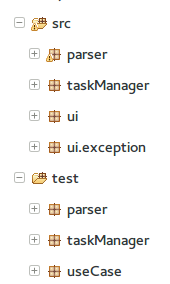
\includegraphics[width=0.25\paperwidth]{figures/Package_overview_eclipse.png}
    \end{column}
    \begin{column}{.5\paperwidth}
   
    \end{column}
\end{columns}
\end{frame}

\begin{frame}
\frametitle{Overview Projectmanagement}

\begin{itemize}
    \item Design co\"ordinator: Andr\'e
    \item Domain co\"ordinator: Thomas
    \item Test co\"ordinator: Bruno
\end{itemize}

Volgende iteratie:

\begin{itemize}
    \item Design co\"ordinator: Bruno
    \item Domain co\"ordinator: Menno
    \item Test co\"ordinator: Thomas
\end{itemize}

\begin{figure}

\end{figure}

\end{frame}

\end{document} 

